\chapter{Przegląd wybranych algorytmów i innych rozwiązań}
\label{cha:rozdz3}

W tym rozdziale przedstawiam algorytmy definiujące funkcję wyboru. Są to kolejno: losowy, zachłanny, minimaksowy oraz Monte Carlo Tree Search. Dla każdego z nich opisuję jego użycie w odniesieniu do gry 'Love Letter'. Ponieważ wszystkie algorytmy będą implementowane w aplikacji komputerowej, przedstawiłem je również w postaci pseudokodu.

\section{Algorytm losowy}
\label{sec:algLos}
\subsection{Opis}
Jest to najprostszy algorytm podejmowania decyzji. Na wejściu otrzymuje listę dostępnych zagrań, z których w całkowicie losowy sposób wybiera jedno. Każde z dostępnych zagrań ma takie samo prawdopodobieństwo wyboru przez ten algorytm.

\subsection{Sposób wykorzystania}
Z uwagi na prostotę algorytmu jest on wykorzystany głównie do przetestowania poprawności działania implementacji gry. Zastosowałem w nim jedną drobną modyfikację: nigdy nie podejmie decyzji o zagraniu Księżniczki - oznacza to natychmiastową przegraną niezależnie od momentu gry, co wypaczałoby wyniki porównań algorytmów.

\subsection{Zapis pseudokodem}
\begin{algorithmic}[1]
	\Function{$d_{losowa}$}{$I_n, X_n$}	
		\ForAll{ $z_i \in X_n$ } \Comment $i = |X_n|$
			\If {$z_i ==$ Księżniczka}
				\State $X_n \gets X_n - z_i$
			\EndIf
		\EndFor
	\State \textbf{return} wylosujJeden($X_n$) 
	\EndFunction
\end{algorithmic}

\section{Algorytm zachłanny}
\label{sec:algZach}
\subsection{Opis}
Algorytm zachłanny polega na wyborze najlepszego możliwego zagrania dostępnego w danej chwili, nie analizując jego konsekwencji w przyszłości. Pomimo, że takie podejmowanie decyzji jest krótkowzroczne, to jest też łatwe w implementacji i daje atrakcyjne wyniki w niektórych problemach, np. przy szukaniu minimalnego drzewa rozpinającego\textsuperscript{[\ref{bib:algorytmy_zachlanny}]}.

\subsection{Sposób wykorzystania}

W kontekście gry 'Love Letter', implementacja algorytmu zachłannego wymaga pewnego doprecyzowania. Najważniejszą częścią jest funkcja kryterialna oceniająca wartość zagrania, która w niektórych przypadkach musi być oparta o prawdopodobieństwo wystąpienia kart u przeciwnika. Prawdopodobieństwo to uzależnione jest od stanu początkowego danej tury.

Rozważmy przypadek, w którym algorytm musi podjąć decyzję o zagraniu karty Strażniczki, lub karty Barona. Jest to pierwszy ruch gracza, a w widocznych kartach odrzuconych na starcie są odrzucone karty Króla, Księcia i Pokojówki. Oznacza to, że w talii pozostało 9 kart, a jedna z odrzuconych jest niewidoczna, niemniej jednak ją też trzeba brać pod uwagę. Wyliczenie prawdopodobieństwa \textit{P[]} jaką kartę ma przeciwnik jest tym momencie proste, jednak trzeba jeszcze wziąć pod uwagę drobny szczegół - czy do liczenia \textit{P[]} wliczać karty posiadane w ręce. Z jednej strony wydaje się to nielogiczne i może prowadzić do wybierania nieoptymalnych decyzji (co przeczyłoby idei algorytmu zachłannego), z drugiej strony można to potraktować jako element blefu, który jest nieodłączną częścią każdej gry towarzyskiej. W swojej implementacji założyłem absolutną zachłanność algorytmu i karty posiadane na ręce są pomijane w obliczeniach. 
Wobec powyższego, prawdopodobieństwa wystąpienia kart u przeciwnika wynikające z ustalonego stanu początkowego są następujące:

\begin{table}[h]
	\caption{Przykład rozkładu prawdopodobieństwa}
	\centering
		\begin{tabular}{|l|r|}
			\hline
			\bf{Karta} & $P[]$	\\ \hline
			Strażniczka & 30\% 			\\ \hline
			Kapłan & 20\% 				\\ \hline
			Baron & 10\% 				\\ \hline
			Pokojówka & 10\% 			\\ \hline
			Książę & 10\% 				\\ \hline
			Hrabina & 10\% 				\\ \hline
			Księżniczka & 10\% 			\\ \hline
		\end{tabular}
\end{table}

Zagranie karty Baron oznacza porównanie drugiej karty z kartą przeciwnika. Łatwo policzyć, że w 70\% przypadków skończyłoby to się porażką, a w 30\% nie było by żadnego efektu. Drugim dostępnym ruchem jest zagranie karty Strażniczki, a w jej przypadku najlepszym wyborem jest wytypowanie Kapłana, co daje 20\% szans na zwycięstwo i 80\% szans, że nie nastąpi żaden efekt. Zauważmy, że gdybyśmy wliczali posiadane karty do obliczenia prawdopodobieństwa, wystąpienie Barona i Kapłana byłoby tak samo możliwe. W takich przypadkach algorytm powinien zawsze celować w kartę z wyższym numerem. By formalnie stwierdzić, jaka decyzja $z$ powinna zostać podjęta, musimy obliczyć funkcję kryterialną dla dostępnych zagrań i wybrać to zagranie, dla której funkcja przyjmuje wyższą wartość. Przyjmijmy, że funkcja kryterialna wygląda następująco:

\begin{center}
	$F(z) = 1 + prawdopodobienstwo\_wygranej - prawdopodobienstwo\_przegranej$
\end{center}
Po podstawieniu otrzymujemy:
\begin{center}
 $F(Str\_Kap)=1.2$ i $F(Bar) = 0.3$
 
 $F(Str\_Kap)>F(Bar) => z = Str\_Kap$ 
\end{center} 

Najlepszą decyzją w tym wypadku jest zagranie karty Strażniczki z wyborem karty Kapłana. Jak jednak na podstawie powyższego wzoru ocenić zagranie karty Kapłana, Pokojówki lub Króla? Każda z nich wymaga indywidualnej oceny. Mając na uwadze, że w kontekście strategii zachłannej decyzja zawsze powinna być optymalna w ujęciu chwili, ustaliłem następujące wskazówki którymi się kierowałem przy tworzeniu funkcji kryterialnej dla zagrań każdej z kart:
\begin{itemize}
	\item Strażniczka - ocena zagrania wzrasta gdy pozwala wyeliminować przeciwnika.
	\item Kapłan - efekt karty jest neutralny i ocena jego zagrania będzie zawsze stała.
	\item Baron - ocena zagrania wzrasta gdy mamy drugą kartę silniejszą niż może mieć przeciwnik i maleje gdy jest odwrotnie.
	\item Pokojówka - podobnie jak w przypadku kapłana, ocena zagrania karty będzie stała.
	\item Książę - ocena zagrania na przeciwnika wzrasta z prawdopodobieństwem Księżniczki u przeciwnika. Ocena zagrania na siebie jest stała, lecz 0 gdy druga karta to Księżniczka.
	\item Król - jak w przypadku kapłana i pokojówki, ocena zagrania jest stała.
	\item Hrabina - ocena stała, jednak musimy ją zagrać gdy druga posiadana karta to Król lub Książę.
	\item Księżniczka - nie może być nigdy wyrzucona.
	\item Dodatkowo, jeśli oba zagrania mają taką samą wartość, powinna być podjęta decyzja o zagraniu karty o niższej wartości $W$, w związku z tym ocena zagrania spada wraz z wyższą wartością karty.
\end{itemize}
Opierając się na powyższych wytycznych, zapisałem algorytm w formie pseudokodu.
\subsection{Zapis pseudokodem}
Wykorzystane zmienne pomocnicze:
\begin{itemize}
	\item $P[]$ - tablica prawdopodobieństwa wystąpienia karty u przeciwnika
	\item $decyzja$ - zagranie, które ma zostać zwrócone
\end{itemize}
\begin{algorithmic}[1]
	\Function{$d_{zachlanna}$}{$I_n, X_n$}
		\State $P[] \gets$ obliczPrawdopodobienstwo()
		\State $ decyzja \gets NULL$ \Comment Szukanie zagrania o najwyższej wycenie
		\ForAll{ $z_i \in X_n$ } \Comment $i=|X_n|$
				\If {$F(decyzja, P[]) < F(z_i, P[]$}
					\State $decyzja \gets z_i$
				\EndIf
		\EndFor		
		\State \textbf{return} $decyzja$
	\EndFunction
\end{algorithmic}

Gdzie funkcja kryterialna wygląda następująco:
\begin{algorithmic}[1]
	\Function{$F$}{$z,P[]$}	
		\Switch{$z$}
			\Case{Str\_Kap} \Comment Zagranie Strażniczki na dany typ karty
				\State \textbf{return} $ 1 + P[Kaplan] + 0.008 $
			\EndCase
			\Case{Str\_Bar}
				\State \textbf{return} $ 1 + P[Baron]  + 0.008 $
			\EndCase
			\State ...
			\Case{Str\_K-a}
				\State \textbf{return} $ 1 + P[Ksiezniczka]  + 0.008 $
			\EndCase
			\Case{Kap\_Z}
				\State \textbf{return} $ 1 + 0.007 $
			\EndCase
			\Case{Bar\_Z}	\Comment Kryterium zależy od wartości $W(DK)$
				\State $ szansePrzegranej \gets 0$ 
				\State $ szanseWygranej \gets 0$ 
				\ForAll {$typKarty$}
					\If {$ W(DK) < W(typKarty) $}  
						\State $szansePrzegranej \gets szansePrzegranej + P[typKarty]$ 
					\ElsIf {$ W(DK) > W(typKarty) $}
						\State $szanseWygranej \gets szanseWygranej + P[typKarty]$ 
					\EndIf
				\EndFor
				\State \textbf{return} $ 1 - szansePrzegranej + szanseWygranej + 0.006 $
			\EndCase
			\Case{Pok\_Z}
				\State \textbf{return} $ 1 + 0.005 $
			\EndCase
			\Case{K-e\_S}
				\State \textbf{return} $ 1 + P[\textit{K-a}] + 0.004 $
			\EndCase
			\Case{K-e\_P} 
				\If {$ DK == $ K-a}  
					\State \textbf{return} $ 0 $
				\Else
					\State \textbf{return} $ 1 + 0.004 $
				\EndIf
			\EndCase
			\Case{Krl\_Z}
				\State \textbf{return} $ 1 + P[\textit{K-a}] + P[Hra] + 0.003 $
			\EndCase
			\Case{Hra\_K-e\_Kr}
				\State \textbf{return} $ 10 + 0.002 $
			\EndCase
			\Case{Hra\_Z}
				\State \textbf{return} $ 1 + 0.002 $
			\EndCase
			\Case{K-a\_Z}
				\State \textbf{return} $ 0 $
			\EndCase
		\EndSwitch
	\EndFunction
\end{algorithmic}


\section{Algorytm min-max}
\label{sec:minmax}
\subsection{Opis}
Algorytm minimaksowy polega na ,,minimalizowaniu maksymalnych możliwych strat'' bądź alternatywnie na ,,maksymalizacji minimalnego zysku (wypłaty)''$^{[\ref{bib:wiki_minMax}]}$. Zgodnie z [\ref{bib:wazniak_minMax}] często stosuje się go do gier o następujących zasadach:
\begin{itemize}
	\item występuje dwóch graczy
	\item ruchy wykonywane są naprzemiennie
	\item w każdym stanie istnieje skończona liczba decyzji do podjęcia
	\item stan i podjęta decyzja jednoznacznie wyznaczają stan następny
	\item każdy stan może zakwalifikować do jednej z następujących kategorii:
	\begin{itemize}
		\item wygrana pierwszego gracza
		\item wygrana drugiego gracza
		\item remis
		\item sytuacja nierozstrzygnięta
	\end{itemize}
\end{itemize}
Najczęstsze implementacje polegają na przeszukiwaniu drzewa dalszych przebiegów gry począwszy od zadanego stanu początkowego, tak jak na przykład w warcabach$^{[\ref{bib:minMax_warcaby}]}$. Istnieją także implementacje opierające się na liczbowej ocenie ruchu$^{[\ref{bib:wazniak_minMax}]}$ i na tej idei opieram swoją implementacje algorytmu minimaksowego.

\subsection{Sposób wykorzystania}
W podanym powyżej opisie, gra Love Letter niezgodna jest w punkcie czwartym. Jak ustaliliśmy wcześniej, gracz nie wie w jakim dokładnie stanie znajduje się gra, zna natomiast zbiór informacyjny $I_n$. Z tego względu, z perspektywy gracza $P_1$ podjęcie decyzji $z_i \in X_n$ nie określa jednoznacznie następnego węzła, lecz loterię. Mimo to, jesteśmy w stanie statystycznie ocenić możliwości przeciwnika, a tym samym zminimalizować naszą maksymalną stratę. Ponieważ zysk należy rozumieć jako zwiększenie szansy na wygraną (tak jak w strategii zachłannej), to strata oznacza zwiększenie szansy na przegraną. 

Rozważmy scenariusz, w którym gracz pierwszy posiada kartę Księcia oraz Pokojówki. Na stosie pozostało 2 karty, 1 karta jest zakryta zgodnie z zasadami rozpoczęcia rundy i przeciwnik również posiada 1 kartę. Wśród tych 4 nieznanych graczowi kart są karty Strażniczki, Barona, Księcia oraz Księżniczki. Prawdopodobieństwo wystąpienia każdej z nich u przeciwnika wynosi 25\% i razem stanowią one tablicę prawdopodobieństwa $P[]$. Przyjmijmy, że wykorzystywana w poprzedniej strategii funkcja kryterialna $F(z, P[])$ to maksymalizacja zysku i nazwijmy ją $F_{max}(z, P[])$  Zgodnie z jej definicją $F_{max}(\textit{K-e}, P[]) = 1.29$ i $F_{max}(Pokojowka, P[]) = 1.05$, więc zagranie Księcia maksymalizuje szansę na wygraną. Jeśli jednak weźmiemy pod uwagę, że w 75\% przypadków nie wygrywamy, wówczas musimy rozważyć odpowiedź przeciwnika. W tym wypadku jest 6 par kart które może posiadać przeciwnik, więc dla każdej z nich, zgodnie ze strategią zachłanną, należy obliczyć funkcję kryterialną oraz szansę na przegraną. Dodatkowo należy zauważyć, że z perspektywy przeciwnika w każdym przypadku gracz pierwszy ma inny rozkład prawdopodobieństwa wystąpienia karty. Pełne obliczenia znajdują się w tabeli poniżej.

\clearpage
\begin{center}
	Gracz pierwszy po zagraniu Księcia posiada tylko kartę Pokojówki. $F(z_1)$ oznacza ocenę zagrania pierwszej karty, $F(z_2)$ oznacza ocenę zagrania drugiej karty.
\end{center}
\begin{table}[h]
	\caption{Scenariusze reakcji przeciwnika na decyzję}
	\centering
	\begin{tabular}{|l|c|r|r|r|}
		\hline
		\bf{Karty 1 i 2} & $P[]$ pierwszego gracza  & $F(z_1)$ & $F(z_2)$ & Szanse przegranej	\\ \hline
		Str ; Bar & $P[\textit{Pok}] = P[\textit{K-e}] = P[\textit{K-a}] = 33.(3)\%$ & 1.41 & 0.6	& 33.(3)\% \\ \hline
		Str ; K-e & $P[\textit{Pok}] = P[\textit{Bar}] = P[\textit{K-a}] = 33.(3)\%$ & 1.41 & 1.37 & 33.(3)\%	\\ \hline
		Str ; K-a & $P[\textit{Str}] = P[\textit{Bar}] = P[\textit{K-e}] = 33.(3)\%$ & 1.41 & 0 & 33.(3)\% \\ \hline
		Bar ; K-e & $P[\textit{Str}] = P[\textit{Pok}] = P[\textit{K-a}] = 33.(3)\%$ & 1.39 & 1.37 & 100\% \\ \hline
		Bar ; K-a & $P[\textit{Str}] = P[\textit{Pok}] = P[\textit{K-e}] = 33.(3)\%$ & 2.06 & 0 & 100\% \\ \hline
		K-e ; K-a & $P[\textit{Str}] = P[\textit{Pok}] = P[\textit{Bar}] = 33.(3)\%$ & 1.04 & 0 & 0\% \\ \hline
	\end{tabular}
\end{table}
Dodatkowo, wprowadźmy funkcję $K(z) = F_{max} - F_{min}$, która wyceni dane zagranie.

Każdy rozważany scenariusz ma taką samą szansę wystąpienia, czyli $\frac{1}{6}$. Statystycznie szansa na przegraną wynosi więc:
\begin{center}
 $\frac{1}{6} * (\frac{1}{3} + \frac{1}{3} + \frac{1}{3} + 1 + 1 + 0) = \frac{1}{6} * 3 = 0.50 $
\end{center}
Warunkiem wystąpienia możliwości przegrania, jest brak wygranej po zagraniu Księcia na przeciwnika, czyli ostatecznie szanse na przegraną wynoszą:
\begin{center}
	$F_{min}(\textit{K-e\_P}, P[]) = 0.75 * 0.50 = 0.375$
\end{center}
Modyfikując o tę wartość ocenę zagrania Księcia otrzymujemy finalnie:
\begin{center}
	$K(\textit{K-e\_P}) =  F_{max}(\textit{K-e\_P}, P[]) - F_{min}(\textit{K-e\_P}, P[]) = 1.29 - 0.375 = 0.915$
\end{center} 
W przypadku zagrania Pokojówki szanse przegrania wynoszą 0\%, ponieważ zgodnie z zasadami gry jesteśmy odporni na działanie kart przeciwnika:
\begin{center}
	$K(Pok\_Z) =  F_{max}(Pok\_Z, P[]) - F_{min}(Pok\_Z, P[]) = 1.05 - 0 = 1.05$
\end{center} 
Wynika z tego, że decyzją która minimalizuje maksymalną stratę jest zagranie $z = Pok\_Z$.

Na podstawie powyższych rozważań zapisałem implementację algorytmu zachłannego w postaci pseudokodu.
\subsection{Zapis pseudokodem}
Wykorzystane zmienne pomocnicze:
\begin{itemize}
	\item $K[z]$ - oznacza wspomnianą wyżej funkcję wyceny zagrania. 
	\item $Y_n$ - oznacza zbiór zagrań dostępnych dla przeciwnika.
	\item $L[Y_n]$ - lista możliwych zbiorów decyzji przeciwnika.
	\item Funkcja $R(L[Y_n])$ oznacza szansę porażki po reakcji przeciwnika.
	\item $RK$ - zbiór zagrań będących reakcją przeciwnika.
	\item $P_{porazki}[]$ - tablica zawierająca prawdopodobieństwo porażki po danym zagraniu
\end{itemize}

\begin{algorithmic}[1]
	\Function{$D_{minimaksowa}$}{$I_n, X_n$}
	\State $P[] \gets$ obliczPrawdopodobienstwo()
		\ForAll{ $z_i \in X_n$ } \Comment $i=|X_n|$
			\State $K[z_i] \gets F_{max}(z_i, P[]) - F_{min}(z_i, P[])$
		\EndFor		
		\State $ decyzja \gets z_0$ \Comment Szukanie zagrania o najwyższej wycenie
		\ForAll{ $z_i \in X_n $ } 
			\If {$K[decyzja] < K[z_i]$}
				\State $decyzja \gets z_i$
			\EndIf
		\EndFor		
		\State \textbf{return} $decyzja$
	\EndFunction
\end{algorithmic}

Funkcja $F_{max}(z, P[])$ jest identyczna do $F(z, P[])$ występującej w strategii zachłannej, w związku z czym zapiszę wyłącznie $F_{min}(z, P[]$).
\begin{algorithmic}[1]
	\Function{$F_{min}$}{$z, P[]$}	
		\State $L[Y_n] \gets$ utwórz listę możliwych zbiorów decyzji u przeciwnika 
		\Switch{$z$}
			\Case{Str\_Kap} \Comment Szanse, że Strażniczka \textbf{nie} przyniesie zwycięstwa
				\State \textbf{return} $ (1 - P[Kap]) * R(L[Y_n]) $
			\EndCase
			\Case{Str\_Bar}
				\State \textbf{return} $ (1 - P[Bar]) * R(L[Y_n]) $
			\EndCase
				\State ...
			\Case{Str\_K-a}
				\State \textbf{return} $ (1 - P[\textit{K-a}]) * R(L[Y_n]) $
			\EndCase
			\Case{Kap\_Z}
				\State \textbf{return} $  R(L[Y_n]) $
			\EndCase
			\Case{Bar\_Z}	\Comment Szanse, że porównanie zakończy się remisem 
				\State $ szanseRemisu \gets P[DK]$ 
				\State \textbf{return} $ szanseRemisu * R(L[Y_n]) $
			\EndCase
			\Case{Pok\_Z}
				\State \textbf{return} $ 0 $
			\EndCase
			\Case{K-e\_P}
				\State \textbf{return} $ (1 - P[\textit{K-a}]) * R(L[Y_n]) $
			\EndCase
			\Case{K-e\_S} 
				\If {$ DK == \textit{K-a} $}  
					\State \textbf{return} $ 0 $
				\Else
					\State \textbf{return} $ R(L[Y_n]) $
				\EndIf
			\EndCase
			\Case{Krl\_Z}
				\State \textbf{return} $ R(L[Y_n]) $
			\EndCase
			\Case{Hra\_K-e\_Krl}
				\State \textbf{return} $ R(L[Y_n]) $
			\EndCase
			\Case{Hra\_Z}
				\State \textbf{return} $ R(L[Y_n]) $
			\EndCase
				\Case{K-a}
			\State \textbf{return} $ 10 $
			\EndCase
		\EndSwitch
	\EndFunction
\end{algorithmic}

Funkcja $R(L[Y_n])$ oznacza szansę porażki po reakcji przeciwnika.
\begin{algorithmic}[1]
	\Function{$R$}{$L[Y_n]$}
		\ForAll {$Y_n \in L[Y_n]$}
			\State $P[] \gets$ obliczPrawdopodobienstwo()
			\State $RK \gets RK \cup D_{zachlanna}(Y_n, P[]) $	\Comment Lista potencjalnych reakcji
		\EndFor
		\ForAll {$z_i \in RK$}	\Comment Sprawdzenie szansy porażki, $i=|RK|$
			\Switch{$z_i$}
				\Case{Str\_DK}
					\State $P_{porazki}[z_i] \gets 1$
				\EndCase
				\Case{Bar\_Z}
					\If{$W(DK) < W(DK_{przeciwnika})$}
						\State $P_{porazki}[z_i] \gets 1$
					\Else
						\State $P_{porazki}[z_i] \gets 0$
					\EndIf
				\EndCase
				\Case{K-e\_Z}
					\If{$DK == \textit{K-a}$}
						\State $P_{porazki}[z_i] \gets 1$
					\Else
						\State $P_{porazki}[z_i] \gets 0$
					\EndIf
				\EndCase
				\Case{default}
					$P_{porazki}[z_i] \gets 0$
				\EndCase
			\EndSwitch
		\EndFor
		\State \textbf{return} $ \sum_{i=0}^{|RK|} \frac{1}{|RK|} * P_{porazki}[i] $
	\EndFunction
\end{algorithmic}


\section{Algorytm Monte Carlo Tree Search}
\label{sec:mcts}

\subsection{Opis}

Drzewo Przeszukiwań Monte Carlo jest metodą heurystycznego podejmowania decyzji, często wykorzystywaną w grach typu Hex$^{[\ref{bib:mcts_hex}]}$ czy Go$^{[\ref{bib:wiki_mcts}]}$. W przeciwieństwie do deterministycznych algorytmów przeszukujących drzewo decyzyjne, MCTS buduje drzewo wariantów poprzez losowe próbkowanie najbardziej obiecujących ruchów. Dzięki temu jego dużą zaletą jest możliwość efektywnego wykorzystania w grach o wysokim rozgałęzieniu drzewa decyzyjnego$^{[\ref{bib:mcts_wprowadzenie}]}$. Popularność wykorzystania tego algorytmu stale rośnie, czego przykładem jest zastosowanie w niedeterministycznej gry planszowej Osadnicy z Catanu$^{[\ref{bib:mcts_osadnicy}]}$, czy w strategii turowej Total War: Rome II$^{[\ref{bib:mcts_totalWar}]}$. Główne cechy algorytmu:
\begin{itemize}
	\item przerywalność algorytmu w dowolnym momencie
	\item zależność wydajności od czasu - im dłużej działa algorytm, tym lepsze osiąga wyniki
	\item uniwersalność - algorytm do działania potrzebuje wyłącznie zbioru dostępnych ruchów oraz możliwości przeprowadzenia losowej rozgrywki od danego stanu
	\item niezależność od wiedzy eksperckiej występującej w grze
\end{itemize}

\subsection{Sposób wykorzystania}

Jak opisali autorzy artykułu \textit{Monte-Carlo Tree Search: A New Framework for Game AI}$^{[\ref{bib:mcts_opis}]}$, zasady działania algorytmu są następujące: otrzymując zbiór informacyjny $I_n$ oraz zbiór dopuszczalnych ruchów (decyzji) $X_n$, tworzony jest korzeń $T$, oraz węzły $s_0$ .. $s_i$ ($i=|X_n|$) odpowiadające stanom gry po wykonaniu dostępnych ruchów (decyzji). Następnie przez zadany czas $t$ powtarzane są następujące kroki:
\begin{enumerate}
	\item \textbf{Selekcja} - zaczynając od korzenia $T$, wybieraj kolejne węzły balansując pomiędzy \textbf{eksploatacją} i \textbf{eksploracją}, aż dotrzesz do węzła-liścia $L$.
	\item \textbf{Ekspansja} - jeśli wybór L nie kończy gry, utwórz węzły potomne i wśród nich wylosuj węzeł $C$
	\item \textbf{Symulacja} - dla wybranego węzła przeprowadzać losową symulację, aż do osiągnięcia wyniku.
	\item \textbf{Propagacja wsteczna} - każdy węzeł od $C$ do $L$ jest aktualizowany o wartość wyniku.
\end{enumerate}
\begin{figure}[h]
	\centering
	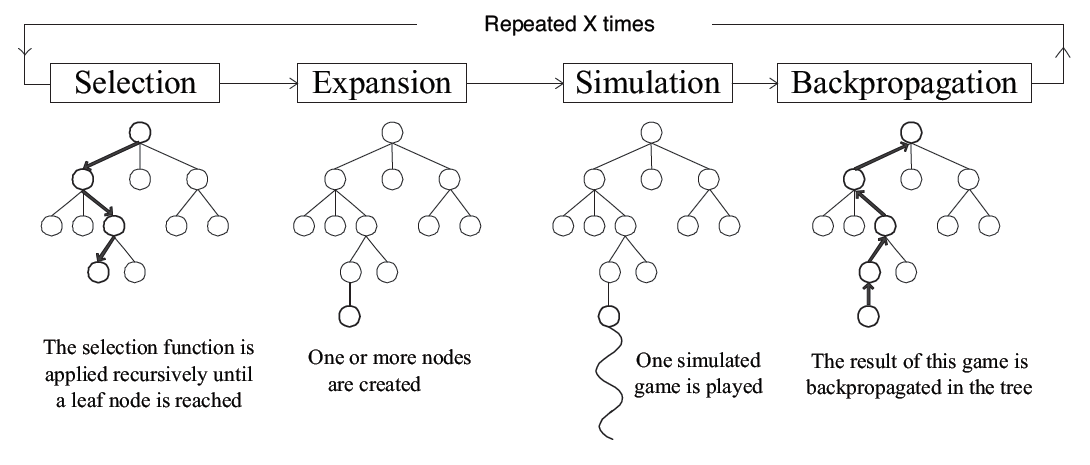
\includegraphics[width=\textwidth]{Resources/mcts.png}
	\caption{Schemat działania algorytmu MCTS$^{[\ref{bib:mcts_opis}]}$} 
	\label{fig:llMainImage}
\end{figure}
Szczególnym elementem jest selekcja. Eksploatacja oznacza wybieranie ruchów o wysokiej częstości wygranych, a eksploracja to badanie ruchów o niskiej liczbie przeprowadzonych symulacji. Brak równowagi pomiędzy tymi dwoma strategiami próbkowania doprowadzi do zakłamań, na przykład poprzez pułapkę optimum lokalnego. W związku z tym w 2006 roku Kocsis i Szepervari opracowali wzór równoważący selekcję nazwany Upper Confidence bound applied to Trees(UCT) (górna granica ufności)$^{[\ref{bib:mcts_uct}]}$:
\begin{center}
	${v_i} + C*\sqrt{\frac{\ln{N}}{n_i}}$
\end{center}
\begin{itemize}
	\item $v_i$ - estymowana wartość węzła
	\item $C$ - empirycznie dobierany parametr eksploracji, zazwyczaj $\sqrt{2}$
	\item $N$ - ilość odwiedzin węzła-rodzica
	\item $n_i$ - ilość odwiedzin w danym węźle
\end{itemize}
Ważne jest, że każdy węzeł posiada informację o szacunkowej wartości opartej na wynikach symulacji, oraz o liczbie przeprowadzonych symulacji.

Ze względu na fakt, że algorytm do działania wymaga wyłącznie listy dostępnych ruchów oraz możliwości przeprowadzenia symulacji, jego implementacja do gry ,,Love Letter'' nie wymaga specjalnych modyfikacji. Powyższa wiedza w pełni pozwala na wykorzystanie algorytmu w grze.
\subsection{Zapis pseudokodem}
Wykorzystane zmienne pomocnicze:
\begin{itemize}
	\item $Nast(u, z)$ - funkcja wskazująca następnik węzła $u$ po wyborze zagrania (łuku) $z$.
	\item $X_L$ - zbiór ruchów dostępnych w węźle $L$.
	\item $wynik$ - wypłata gracza po symulacji.
\end{itemize}
\begin{algorithmic}[1]
	\Function{$d_{mcts}$}{$I_n, X_n$}
		\State $T \gets $ utwórz korzeń T z obecnego zbioru informacyjnego $I_n$
		\Repeat
			\State $L \gets $ selekcja($T$)
			\If {$L$ nie jest końcem gry}
				\ForAll{ $z_i \in X_L$ } \Comment $i=|X_L|$, 
					\State $L \gets$ dodajDziecko($Nast(L, z_i)$)
				\EndFor
				\State $C \gets$ wylosujDziecko($L$)
				\State $wynik \gets$ symuluj($C$)	\Comment Symulacja
				\Repeat	\Comment Propagacja wsteczna
					\State $C \gets $ aktualizuj($wynik$)
					\State $C \gets $ rodzic($C$)
				\Until {$C==T$}
			\EndIf 
		\Until{koniec czasu}
		\State $decyzja \gets$ najwięcejSymulacji($R$) \Comment ruch z najbardziej obiecującego węzła 
		\State \textbf{return} $decyzja$
	\EndFunction
\end{algorithmic}